\section{Thực nghiệm}

% ============================================================
% SLIDE S4
% ============================================================
\SectionSlide{04}{CHƯƠNG 4}{Thực nghiệm}{6 datasets, 7 baselines}{%
  \SecItem{4.1}{Độ chính xác (Q1)}
  \SecItem{4.2}{Tốc độ (Q2)}
  \SecItem{4.3}{Khả năng diễn giải (Q3) và ablation}}


% ============================================================
% SLIDE 18
% ============================================================
\begin{frame}{Thiết lập thực nghiệm}{Setup}
\begin{columns}[T,onlytextwidth]
\begin{column}{0.58\textwidth}
\small
\begin{tabular}[t]{@{}llll@{}}
  \toprule
  \# & Dataset & Ví dụ từ khóa & Kích thước \\
  \midrule
  1 & Device & iPhone, Galaxy, iPad\ldots & $676\times8\times50$ \\
  2 & Pythonlib & pandas, numpy, pytorch\ldots & $676\times7\times50$ \\
  3 & VoD & netflix, hulu, youtube\ldots & $676\times7\times50$ \\
  4 & Chatapp & facebook, tiktok\ldots & $676\times8\times50$ \\
  5 & Language & python, Java, SQL\ldots & $676\times9\times50$ \\
  6 & Covid-19 & ca nhiễm / tử vong mới & $990\times2\times50$ \\
  \bottomrule
\end{tabular}\par
\vspace{1mm}
{\scriptsize\color{DTMuted}1--5: Google Trends theo tuần, 2010--2022. 6: theo ngày, 01/2020--09/2022. Tất cả chuẩn hóa về $[0,1]$.}
\end{column}
\begin{column}{0.39\textwidth}
\begin{questioncard}
  \small
  \textbf{Cửa sổ}: $L_c=104$ tuần (Covid: 56 ngày)\\
  \textbf{Dự báo}: $L_f\in\{13,26,39\}$ tuần (Covid: $\{7,14,21\}$ ngày)\\
  \textbf{Metric}: MAE, RMSE
\end{questioncard}
\vspace{2mm}
\begin{questioncard}
  \small\textbf{7 baseline}\\
  Tensor/lan truyền: DISMO, FluxCube\\
  Deep learning: PatchTST, Autoformer, DeepAR, LaST, CoST
\end{questioncard}
\end{column}
\end{columns}
\vspace{3mm}
\begin{intuition}[Ba câu hỏi]
  \small \textbf{Q1} Dự báo có chính xác không? \quad
  \textbf{Q2} Có nhanh không? \quad
  \textbf{Q3} Có trích được động thái diễn giải được không?
\end{intuition}
\vfill
\papersource{§5, Table 4, Appendix B.1.}
\end{frame}

% ============================================================
% SLIDE 19
% ============================================================
\begin{frame}{Q1: Độ chính xác}{Kết quả}
\centering
\small
\begin{tabular}{@{}lc|cc|ccccc@{}}
  \toprule
  Dataset & $L_f$ & \textbf{D-Tracker} & DISMO & FluxCube & PatchTST & Autoformer & DeepAR & CoST \\
  \midrule
  Device    & 26 & \bestcell{0.90} & \secondcell{1.19} & 3.85 & 1.54 & 1.31 & 2.21 & 1.80 \\
  Pythonlib & 26 & \bestcell{0.32} & 0.52 & 0.93 & 0.95 & 0.47 & 2.01 & \secondcell{0.45} \\
  VoD       & 26 & \bestcell{0.59} & \secondcell{0.66} & 2.83 & 0.84 & 0.74 & 1.88 & 2.36 \\
  Chatapp   & 26 & \bestcell{0.34} & \secondcell{0.48} & 1.48 & 0.74 & 0.81 & 2.16 & 2.09 \\
  Language  & 26 & \bestcell{0.35} & 1.12 & 1.42 & 0.50 & \secondcell{0.41} & 2.03 & 0.47 \\
  Covid-19  & 14 & \bestcell{0.70} & 1.33 & 1.97 & 2.04 & \secondcell{1.18} & 2.30 & 1.45 \\
  \bottomrule
\end{tabular}\par
\vspace{1mm}
{\scriptsize\color{DTMuted}MAE ($\times10^{-2}$), bước dự báo giữa. \textbf{Đậm}: tốt nhất; gạch dưới: thứ hai. Lược LaST; bảng đầy đủ ở Appendix A9.\par}

\vspace{2mm}
\begin{columns}[T,onlytextwidth]
\begin{column}{0.48\textwidth}
\begin{takeaway}[Kết quả]
  \small MAE \textbf{tốt nhất trên cả 6 dataset}, mọi $L_f$; tốt hơn \textbf{tới 57\%} (Covid-19, $L_f=7$).
\end{takeaway}
\end{column}
\begin{column}{0.48\textwidth}
\begin{intuition}[Vì sao baseline thua?]
  \small Deep learning học offline nên không kịp theo khi trend đổi.
  DISMO bỏ qua phụ thuộc giữa các vùng và không đổi được rank.
\end{intuition}
\end{column}
\end{columns}
\vfill
\papersource{Table 3, §5 Q1.}
\end{frame}

% ============================================================
% SLIDE 20
% ============================================================
\begin{frame}{Q2: Tốc độ}{Kết quả}
\begin{columns}[c,onlytextwidth]
\begin{column}{0.36\textwidth}
  \centering
  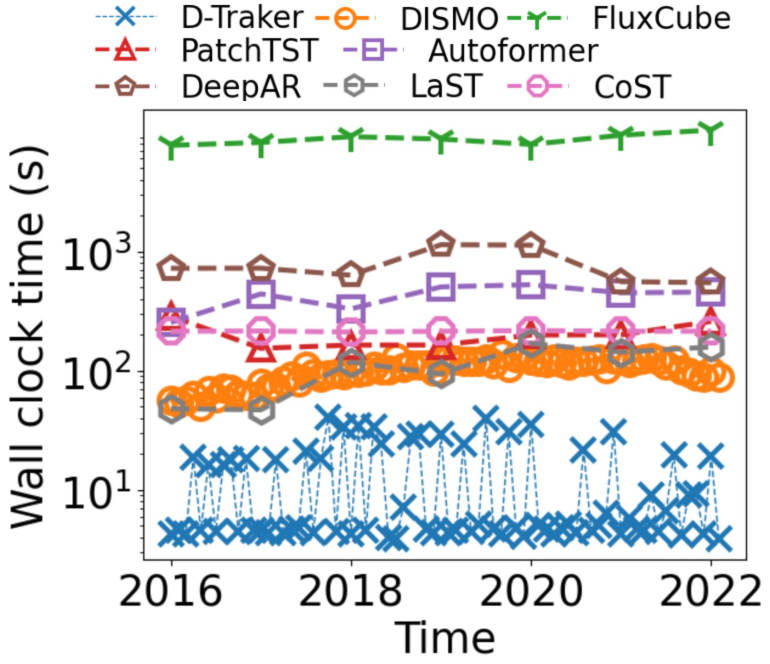
\includegraphics[width=\linewidth]{figures/scalability.png}\par
  {\scriptsize\color{DTMuted}Thời gian mỗi lần cập nhật theo thời gian, Pythonlib (log scale).}
\end{column}
\begin{column}{0.30\textwidth}
  \centering
  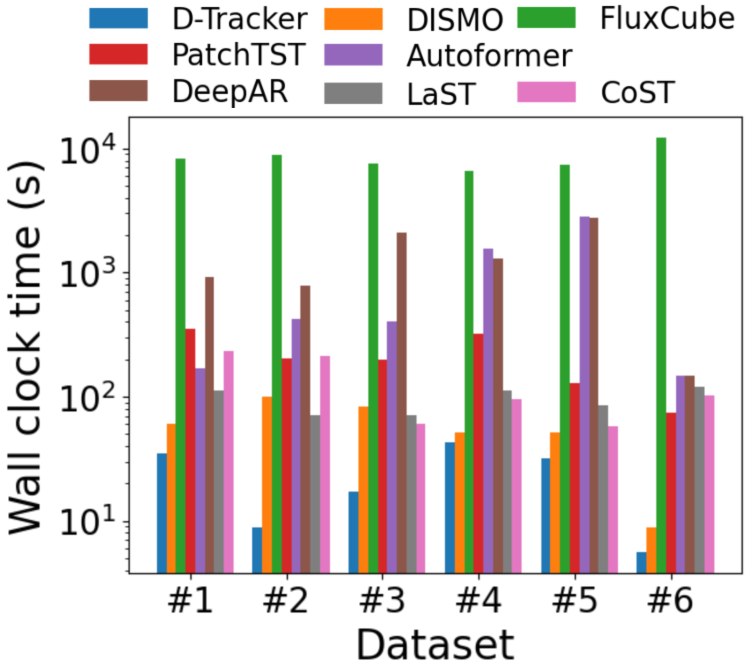
\includegraphics[width=\linewidth]{figures/avgtime.png}\par
  {\scriptsize\color{DTMuted}Thời gian trung bình trên toàn luồng.}
\end{column}
\begin{column}{0.30\textwidth}
  \small
  \begin{itemize}
    \item D-Tracker: \textbf{phẳng} theo độ dài luồng.
    \item Gai nhỏ = lúc RankUpdate chạy.
    \item DISMO chậm dần; FluxCube rất chậm vì phải huấn luyện lại.
  \end{itemize}
  \vspace{2mm}
  \begin{takeaway}[Kết quả]
    \small Nhanh nhất, \textbf{tới 8.0$\times$} so với đối thủ.
  \end{takeaway}
\end{column}
\end{columns}
\vfill
\papersource{Figure 4, §5 Q2, §1.}
\end{frame}

% ============================================================
% SLIDE 21
% ============================================================
\begin{frame}{Q3: Đọc được câu chuyện lan truyền}{Kết quả}
\begin{columns}[c,onlytextwidth]
\begin{column}{0.50\textwidth}
  \centering
  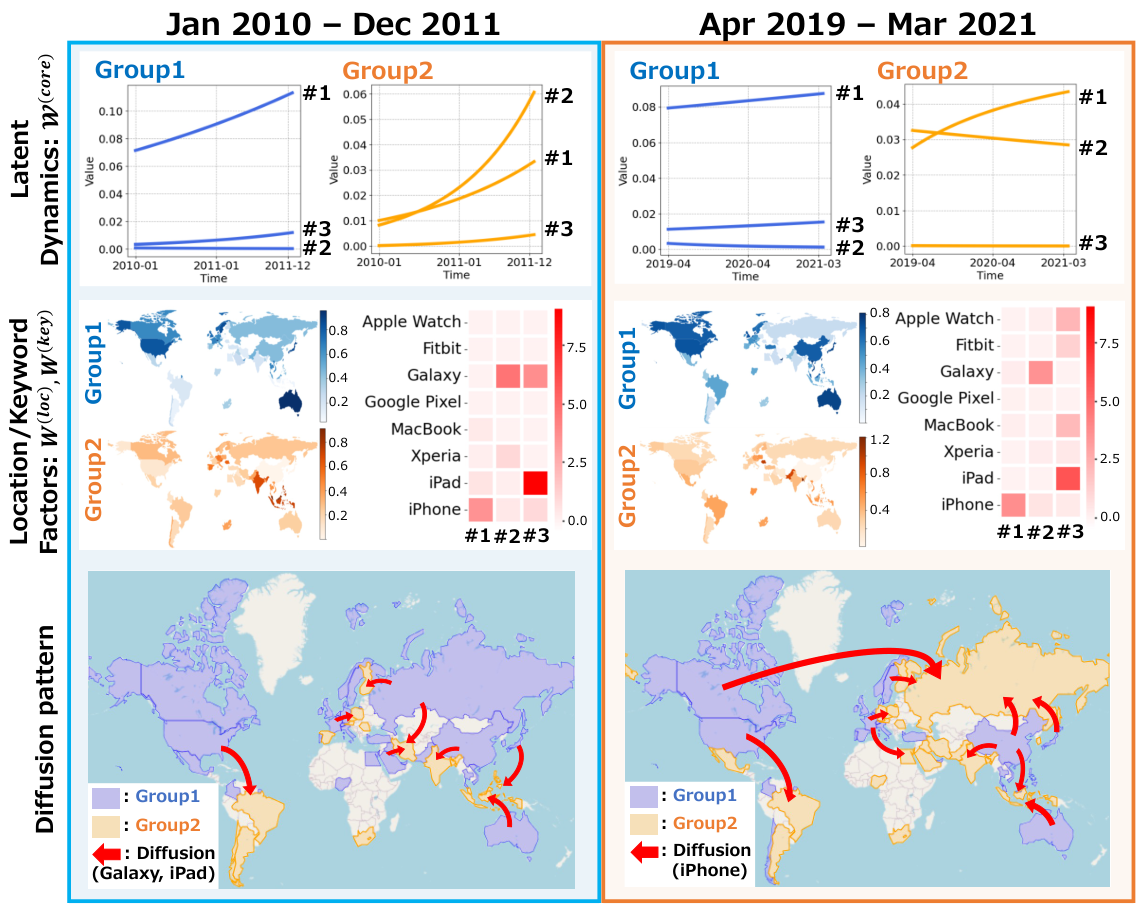
\includegraphics[width=\linewidth,height=0.74\textheight,keepaspectratio]{figures/Figure1_b.png}
\end{column}
\begin{column}{0.47\textwidth}
  \small
  \textbf{Đọc hình theo ba tầng:}
  \begin{enumerate}
    \item Hàng trên: $\mathcal W^{(\mathrm{core})}$, các chuỗi ẩn theo Group 1/2.
    \item Hàng giữa: $W^{(\mathrm{loc})}$ (bản đồ), $W^{(\mathrm{key})}$ (heatmap).
    \item Hàng dưới: hướng lan suy ra từ $\mathcal D$.
  \end{enumerate}
  \vspace{1mm}
  \begin{questioncard}
    \small\textbf{2010--2011}: Dynamics \#2 (``Galaxy'') tăng mạnh ở Đông Nam Á và Nam Mỹ; \#3 (Galaxy, iPad) lan Group 1 $\rightarrow$ 2.\par
    \vspace{1mm}
    \textbf{2019--2021}: \#1 (``iPhone'') lan từ Mỹ, châu Âu, Trung Quốc $\rightarrow$ phần còn lại.
  \end{questioncard}
  {\scriptsize Tương tự, Pythonlib: ``pandas'' lan từ Bắc Mỹ/Úc sang châu Á (Figure 5).\par}
  \vspace{1mm}
  {\small\color{DTGold!80!black}\textbf{Điểm khác biệt:} PatchTST hay DeepAR không trả lời được \emph{ai lan sang ai}.\par}
\end{column}
\end{columns}
\vfill
\papersource{§1.1, Figure 1(b); §5 Q3, Figure 5.}
\end{frame}

% ============================================================
% SLIDE 22
% ============================================================
\begin{frame}{Ablation: thành phần nào có ích?}{Kết quả}
\begin{columns}[c,onlytextwidth]
\begin{column}{0.58\textwidth}
  \centering
  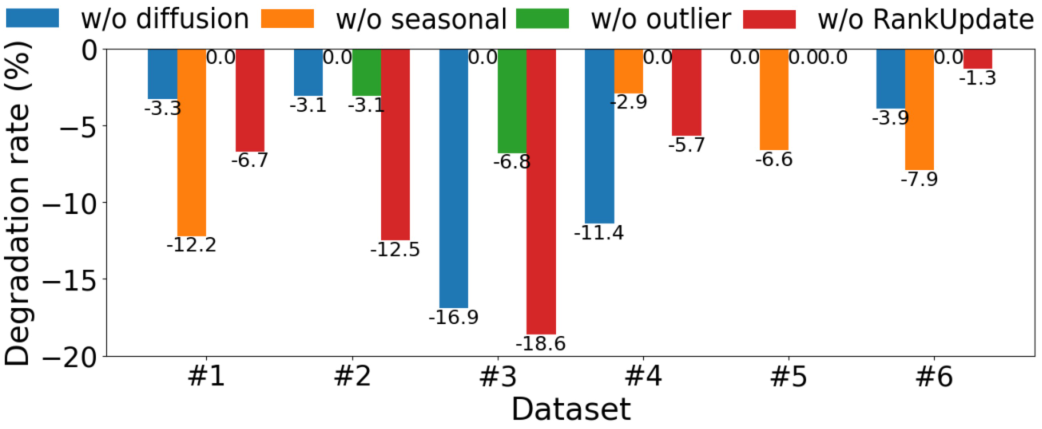
\includegraphics[width=\linewidth]{figures/drop_rate.png}\par
  {\scriptsize\color{DTMuted}Mức giảm MAE khi bỏ từng thành phần ($L_f=26$ tuần / 14 ngày). \#1 Device \ldots\ \#6 Covid-19.}
\end{column}
\begin{column}{0.39\textwidth}
  \small
  \begin{itemize}
    \item Bỏ \textbf{diffusion}: VoD $-16.9\%$, Chatapp $-11.4\%$.
    \item Bỏ \textbf{seasonal}: Device $-12.2\%$, Covid $-7.9\%$, Language $-6.6\%$.
    \item Bỏ \textbf{RankUpdate}: VoD $-18.6\%$, Pythonlib $-12.5\%$.
    \item Bỏ \textbf{outlier}: VoD $-6.8\%$, Pythonlib $-3.1\%$.
  \end{itemize}
  \vspace{1mm}
  \begin{intuition}[Đọc kết quả]
    \small Dataset không có mẫu nào thì thành phần đó cho $0\%$; vd Language gần như không có lan truyền.
  \end{intuition}
\end{column}
\end{columns}
\vfill
\papersource{Figure 3, §5.}
\end{frame}

% ============================================================
% SLIDE 23
% ============================================================
\begin{frame}{Takeaways và hạn chế}{Tổng kết}
\begin{columns}[T,onlytextwidth]
\begin{column}{0.47\textwidth}
  \softlabel{MANG VỀ}\par\vspace{1mm}
  \begin{takeaway}[Interpretable]
    \small Tucker + ODE phản ứng--khuếch tán $\Rightarrow$ đọc được trend và \textbf{lan truyền}.
  \end{takeaway}\par\vspace{1.5mm}
  \begin{takeaway}[Automatic]
    \small MDL tự chọn rank, outlier, thời điểm đổi mô hình.
  \end{takeaway}\par\vspace{1.5mm}
  \begin{takeaway}[Scalable]
    \small Cửa sổ + cập nhật tăng dần $\Rightarrow$ nhanh, không phụ thuộc độ dài luồng.
  \end{takeaway}
\end{column}
\begin{column}{0.50\textwidth}
  \softlabel{HẠN CHẾ / CÂU HỎI MỞ (NHẬN XÉT CỦA NHÓM)}\par\vspace{1mm}
  \small
  \begin{itemize}
    \item Lan truyền giữa \textbf{nhóm vùng ẩn}, không phải giữa từng nước; muốn nói ``Mỹ $\rightarrow$ Việt Nam'' phải đọc qua $W^{(\mathrm{loc})}$.
    \item Số hạng $a\,w$ cho tăng/giảm \textbf{hàm mũ} $\Rightarrow$ dự báo xa có thể bùng nổ hoặc tắt dần nếu không đổi mô hình.
    \item Giả định lan từ cao xuống thấp: sự kiện toàn cầu cùng lúc (trailer, ra mắt đồng loạt) chưa chắc là ``lan truyền''.
    \item Google Trends là chỉ số \textbf{tương đối}, đã chuẩn hóa; không phải số lượt tìm tuyệt đối.
  \end{itemize}
\end{column}
\end{columns}
\vfill
\papersource{§6 Conclusion; hạn chế do nhóm tự nhận xét.}
\end{frame}
